\section{Auswertung}
\label{sec:Auswertung}
Im Folgenden wird die Schallgeschwindigkeit in Acryl als $c_{\text{Acryl}} = \qty{2730}{\metre\per\second}$ und die von destilliertem Wasser als 
$c_{\text{dest.Wasser}} = \qty{1483}{\metre\per\second}$ angenommen. Der verwendete Acrylblock hat eine Gesamthöhe $h_{\text{ges}} = \qty{80.55}{\milli\metre}$. 
Die Fehler zur Bestimmung der Dicke der Kontaktmittelschicht wurden gemäß des Standardfehlers des Mittelwertes durch 
\begin{equation}
  \label{eqn:Fehler}
  \sigma_{\overline{\text{x}}} = \frac{\sigma}{\sqrt{n}}
\end{equation}
berechnet.
Alle anderen Fehler genügen der gaußschen Fehlerfortpflanzung
\begin{equation}
  \label{eqn:Gauss}
  \Delta F = \sqrt{\sum_i\left(\frac{\symup{d}F}{\symup{d}y_i}\Delta y_i \right)^2}.
\end{equation}

\subsection{Abmessungen des Acrylblocks}
\label{subsec:schieblehre}
In \autoref{tab:handmessung} werden die Positionen und Durchmesser der Fehlestellen im Acrylblock aufgefürt. Die Nummerierung der Fehlstellen
und die Bedeutung von \glqq oben\grqq{} und \glqq unten\grqq{} sind \autoref{fig:acrylskizze} zu entnehmen.

\begin{table}[H]
  \centering
  \caption{Mit dem Messschieber bestimmte Realwerte der Abmessungen. $N$ beschreibt die Nummer der Fehlstelle, 
  'o' die Tiefe der Fehlstelle von oben und 'u' die Tiefe der Fehlstelle von unten. $d$ beschreibt den Durchmesser.} 
  \label{tab:handmessung}
  \begin{tabular}{S[table-format = 2.0] S[table-format = 2.2] S[table-format = 2.2] S[table-format = 2.2]}
      \toprule
      {$N$} & {$\symup{o}(N) / \unit{\milli\metre}$} & {$\symup{u}(N) / \unit{\milli\metre}$} & {$d / \unit{\milli\metre}$}\\
      \midrule
      1 & 13.35 & 61.30 & 5.90 \\
      2 & 21.80 & 53.75 & 5.00 \\
      3 & 30.60 & 45.95 & 4.00 \\
      4 & 38.80 & 38.85 & 2.90 \\
      5 & 46.75 & 30.90 & 2.90 \\
      6 & 54.80 & 22.85 & 2.90 \\
      7 & 62.80 & 14.85 & 2.90 \\
      8 & 71.00 &  6.65 & 2.90 \\
      9 & 16.10 & 54.65 & 9.80 \\
     10 & 59.40 & 19.70 & 1.45 \\
     11 & 61.20 & 17.90 & 1.45 \\
     \bottomrule
  \end{tabular}   
\end{table}

\subsection{A-Scan zur Bestimmung der Dicke der Kontaktmittelschicht}
\label{subsec:ascankontakt}
Aus diesen Werten kann nun die theoretische Laufzeit des Ultraschallsignals durch den Acrylblock bestimmt werden. Diese wird gemäß der Formel \eqref{eqn:theorielaufzeit} bestimmt.
\begin{equation}
  \label{eqn:theorielaufzeit}
  t_{\text{Theorie}} = 2 \cdot c_{\text{Acryl}} \cdot o(N)
\end{equation}

Die gemessenen Werte der Laufzeit, welche in \autoref{tab:Messwerte} unterscheiden sich aufgrund der Kontaktmittelschicht von der Theorie. Um diesen Fehler auszubessern wird mittels einer Ausgleichsrechnung die Dicke
der Anpassungsschicht bestimmt. Dazu wird zunächst der Betrag der Differenz zwischen den Theoriewerten und denn Messwerten gebildet. Diese werden dann gemittelt, sodass man einen Mittelwert
und einen Mittelwertfehler\eqref{eqn:Fehler} bestimmen kann. Der Mittelwert der Differenzen mit Fehler ergibt sich zu $\overline{t_{\text{diff}}} = \qty{1.60+-0.07}{\micro\second}$.
Aus diesem Mittelwert kann man nun über das Weg-Zeit-Gesetz \eqref{eqn:WegZeit} und der Gaußschen Fehlerfortpflanzung\eqref{eqn:Gauss} die Dicke der Anpassungsschicht $b_{\text{Anpassungsschicht}}$ bestimmen.
Diese beträgt $b_{\text{Anpassungsschicht}} = \qty{1.19+-0.05}{\milli\metre}$.
\subsection{A-Scan zur Bestimmung der genauen Positionen der Fehlstellen}
\label{subsec:ascanpos}
Nun werden die Laufzeiten für alle Störstellen gemessen. Dabei wird der Acrylblock von beiden Seiten untersucht. Die Messwerte werden in \autoref{tab:Messwerte} dargestellt.
Beim Durchmesser wurde die Laufzeitkorrektur bereits vorgenommen.
\begin{table}
  \centering
  \caption{In dieser Tabelle sind die durch einen A-Scan gemessenen Daten der Fehlstellen aufgeführt. $N$ beschreibt die Lochnummer, \dq o\dq \: die Tiefe der Fehlstelle von 
  oben, \dq u\dq \: die Tiefe der Fehlstelle von unten und $d$ den Durchmesser dieser.} 
  \label{tab:Messwerte}
  \begin{tabular}{S[table-format = 2.0] S[table-format = 2.2] S[table-format = 2.2] S[table-format = 2.2]}
      \toprule
      {$N$} & {$\text{o}(N)$} & {$\text{u}(N)$} & {$d$}\\
      \midrule
      1 & 14.8 & 62.3 &  5.83 \\
      2 & 22.9 & 54.9 &  5.13 \\
      3 & 31.6 & 47.3 &  4.03 \\
      4 & 40.1 & 40.1 &  2.73 \\
      5 & 48.0 & 32.1 &  2.83 \\
      6 & 55.9 & 24.2 &  2.83 \\
      7 & 63.8 & 16.3 &  2.83 \\
      8 &      &  8.4 &       \\
      9 & 16.3 & 56.4 & 10.23 \\
     10 & 60.5 & 20.6 &  1.83 \\
     11 & 62.1 & 19.2 &  1.63 \\
     \bottomrule
  \end{tabular}   
\end{table}

Nun wird noch die Laufzeitkorrektur für die einzelnen Messwerte unternommen. Dazu wird von den gemessenen Laufzeiten $2\cdot \frac{c_{\text{dest.Wasser}}}{b_{\text{Anpassungsschicht}}}$ abgezogen.
Die korregierten Laufzeiten werden nun zusammen mit den theoretischen Laufzeiten mittels des Weg-Zeit-Gesetzes \eqref{eqn:WegZeit} in Tiefen umgerechnet und dann in \autoref{fig:grafik} 
gemeinsam dargestellt.

\begin{figure}
  \centering
\includegraphics[width=\textwidth]{build/plot.pdf}
  \caption{In dieser Grafik sind die experimentell bestimmten Abmessungen der Fehlstellen dargestellt.}
  \label{fig:grafik}
\end{figure}

\subsection{Untersuchung des Auflösungsvermögens}
\label{subsec:auflösung}
Um das Auflösungsvermögen zu Untersuchen werden der Fehlerstellen zehn und elf mit Ultraschallsonden unterschiedlicher Frequenzen untersucht.
Wie man in \autoref{fig:einMHz} erkennt, zeigt diese Sonde nur einen Peak für beide Fehlstellen an. Daher kann nicht eindeutig die Tiefe einer der beiden Fehlstellen bestimmt werden.
Mit der 2MHz-Sonde, wie in \autoref{fig:zweiMHz} zu sehen ist, lässt sich der Peak in zwei nah beieinander liegende Peaks trennen. Anhand dieser Frequenz ist es also möglich 
die einzelnen Tiefen der Fehlstellen zu bestimmen.
\begin{figure}
  \centering
\includegraphics[width=0.5\textwidth]{content/einMHz.pdf}
  \caption{In dieser Grafik wird mit einer 1MHz-Sonde ein A-Scan der Fehlstellen 11 und 12 dargestellt.}
  \label{fig:einMHz}
\end{figure}
\begin{figure}[H]
  \centering
\includegraphics[width=0.5\textwidth]{content/2MHz (unten).pdf}
  \caption{In dieser Grafik wird mit einer 2MHz-Sonde ein A-Scan der Fehlstellen 11 und 12 dargestellt.}
  \label{fig:zweiMHz}
\end{figure}

\subsection{Bestimmung der Fehlstellen über einen B-Scan}
\label{subsec:b_scan}
Mithilfe eines Brightness-Scans kann eine zweidimensionale Aufnahme des Querschnittes des Acrylblockes erstellt werden. Die gesuchten Fehlstellen erscheinen als 
weiße Flächen auf der erzeugten Grafik. Anhand eines Maßstabes können anschließend die Distanzen zwischen den Fehlstellen und der Blockoberseite ermittelt werden.
In den Abbildungen \ref{fig:B_Scan_oben} und \ref{fig:B_Scan_unten} sind die erstellten Aufnahmen zu sehen. Die weiße Linie im unteren viertel der Bilder entspricht
der Unterseite des Blockes, an welcher ein Teil des Ultraschalles reflektiert wird. Anhand dieser Linie und der bekannten Höhe des Acrylwerkstückes lässt sich ein
Maßstab finden, mit welchem die Abstände in Pixeln in metrische Distanzen umgerechnet werden können. Es ist zu beachten, dass zusätzlich zur Höhe des Acrylblockes
die Dicke der Anpassungsschicht $b = \qty{1.19}{\milli\metre}$ addiert werden muss. diese ist als weiße Schicht an der oberen Kante der Bilder zu erkennen.

\begin{figure}
  \centering
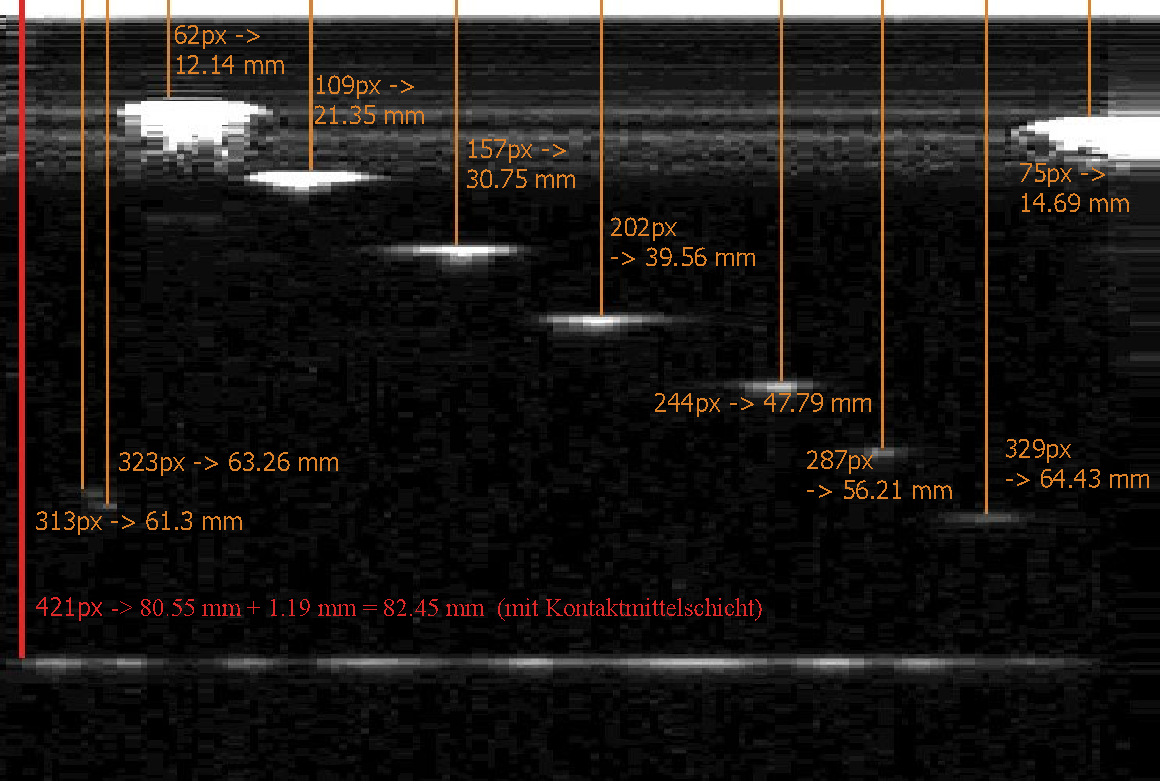
\includegraphics[width=0.7\textwidth]{content/B_Scan_oben_auswertung.pdf}
  \caption{Aufnahme des B-Scans der oberen Seite des Acrylblockes. Die 8. Fehlstelle wurde nicht detektiert.
  Die relevanten Abstände sind an den jeweiligen Fehlstellen markiert.}
  \label{fig:B_Scan_oben}
\end{figure}

\begin{figure}
  \centering
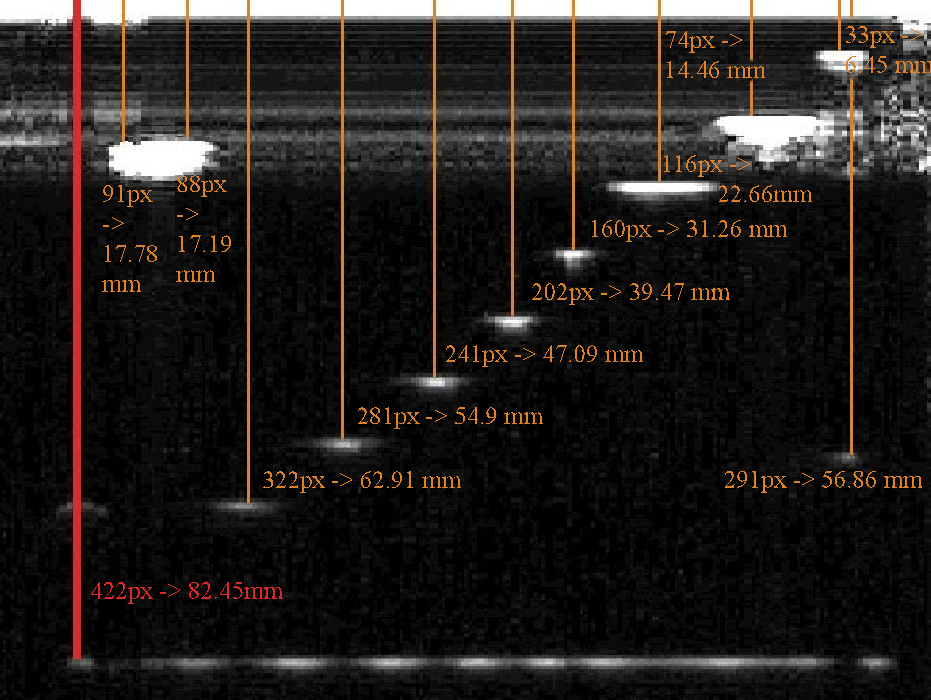
\includegraphics[width=0.7\textwidth]{content/B_Scan_unten_auswertung.pdf}
  \caption{Aufnahme des B-Scans der unteren Seite des Acrylblockes.}
  \label{fig:B_Scan_unten}
\end{figure}

Die grafisch ermittelten Abstände werden in \autoref{tab:B_Scan} gegen die realen Abstände dargestellt. Dabei muss die Dicke der Anpassungsschicht von den in den Abbildungen
\ref{fig:B_Scan_oben} und \ref{fig:B_Scan_unten} dargestellten Werten wieder subtrahiert werden, um den Messwert zu erhalten.
Die relative Abweichung der grafisch ermittelten Werte zu den Realen berechnet sich gemäß
\begin{equation*}
  \symup{\Delta_\text{relativ}}(x) = \frac{|\overline{x} - x|}{\overline{x}},
\end{equation*}
mit Theoriewert $\overline{x}$ und Messwert $x$.

\begin{table}[H]
  \centering
  \caption{Reale Maße der Bohrungen und aus B-Scan ermittelte Längen. 
  o: Abstand zur Oberkante des Acrylblocks, u: untere Kante}
  \label{tab:B_Scan}
  \begin{tabular}{c S[table-format = 2.2] S S S S S}
    \toprule
    {Fehlstelle-Nr.} & {$\symup{o}_\text{real} / \unit{\micro\meter}$}  & {o $ / \unit{\micro\meter}$} & {$\symup{\Delta}_\text{rel}(\text{o}) / \%$} &%
    {$\symup{u}_\text{real} / \unit{\micro\meter}$} & {u $/ \unit{\micro\meter}$} & {$\symup{\Delta}_\text{rel}(\text{u}) / \%$} \\
    \midrule
     1 & 13.35 & 10.95 & 17.98 & 61.3  & 61.72 &  0.69 \\
     2 & 21.8  & 20.16 &  7.52 & 53.75 & 53.71 &  0.07 \\
     3 & 30.6  & 29.56 &  3.40 & 45.95 & 45.9  &  0.11 \\
     4 & 38.8  & 38.37 &  1.11 & 38.85 & 38.28 &  1.47 \\
     5 & 46.75 & 46.6  &  0.32 & 30.9  & 30.07 &  2.69 \\
     6 & 54.8  & 55.02 &  0.40 & 22.85 & 21.47 &  6.04 \\
     7 & 62.8  & 63.24 &  0.70 & 14.85 & 13.27 & 10.64 \\
     8 & 71.0  &       &       &  6.65 &  5.26 & 20.90 \\
     9 & 16.1  & 13.5  & 16.15 & 54.65 & 55.67 &  1.87 \\
    10 & 59.4  & 60.11 &  1.18 & 19.7  & 16.59 & 15.79 \\
    11 & 61.2  & 62.07 &  1.42 & 17.9  & 16.0  & 10.61 \\
    \bottomrule
  \end{tabular}
\end{table}

\subsection{Untersuchung des Brustmodells mit einem B-Scan}
\label{subsec:Brustmodell}
Im letzten Teil des Versuches wird ein B-Scan verwendet, um Tumore in einem Brustmodell ausfindig zu machen. Zuvor wird die ungefähre Position dieser
ertastet, um anschließend einen B-Scan entlang einer Linie über den Tumor durchführen zu können. Beide Tumore sind etwa $1$ bis $\qty{1.5}{\centi\metre}$ groß.

\begin{figure}
  \centering
  \begin{subfigure}{0.4\textwidth}
      \includegraphics[width=\textwidth]{content/tumor1.pdf}
      \caption{B-Scan des ersten Tumors.}
      \label{fig:tumor1}
  \end{subfigure}
  \hfill
  \begin{subfigure}{0.4\textwidth}
    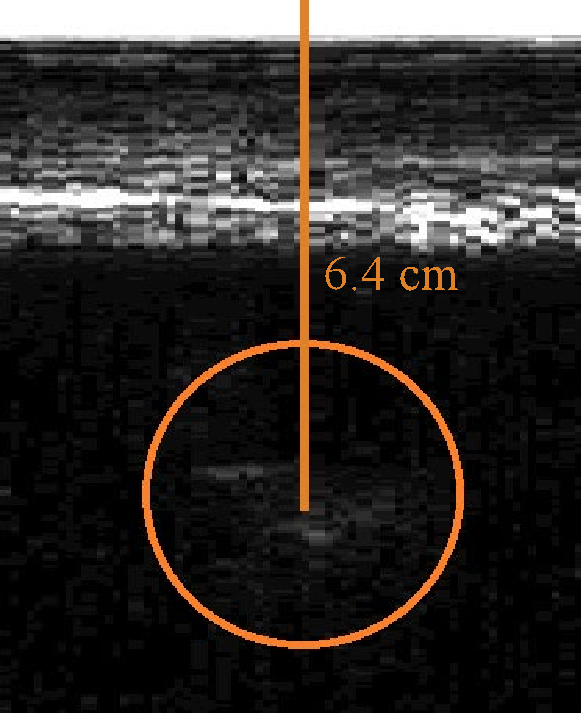
\includegraphics[width=\textwidth]{content/tumor2.pdf}
    \caption{B-Scan des zweiten Tumors.}
    \label{fig:tumor2}
\end{subfigure}     
  \caption{B-Scans der beiden Tumore des Brustmodells. Die orangen Markierungen zeigen die Tumore und deren ungefähre Tiefe.}
  \label{fig:figures}
\end{figure}
